% ****** Start of file aipsamp.tex ******
%
%   This file is part of the AIP files in the AIP distribution for REVTeX 4.
%   Version 4.1 of REVTeX, October 2009
%
%   Copyright (c) 2009 American Institute of Physics.
%
%   See the AIP README file for restrictions and more information.
%
% TeX'ing this file requires that you have AMS-LaTeX 2.0 installed
% as well as the rest of the prerequisites for REVTeX 4.1
%
% It also requires running BibTeX. The commands are as follows:
%
%  1)  latex  aipsamp
%  2)  bibtex aipsamp
%  3)  latex  aipsamp
%  4)  latex  aipsamp
%
% Use this file as a source of example code for your aip document.
% Use the file aiptemplate.tex as a template for your document.
\documentclass[%
 aip,
 % apl,
% jmp,%
% bmf,%
% sd,%
% rsi,%
 amsmath,amssymb,
% preprint,%
 reprint,%
% author-year,%
% author-numerical,%
 floatfix,%
]{revtex4-1}

\usepackage[utf8]{inputenc}
\usepackage{tikz}
\usepackage{graphicx}% Include figure files
\usepackage{dcolumn}% Align table columns on decimal point
\usepackage[T1]{fontenc}
\usepackage{bm}% bold math
\usepackage{mathptmx}
%\usepackage[mathlines]{lineno}% Enable numbering of text and display math
%\linenumbers\relax % Commence numbering lines
\usetikzlibrary{arrows,decorations.markings,decorations.pathmorphing, patterns,shapes}

\begin{document}

\preprint{AIP/123-QED}

\title[]{Head Injury Mechanics:\\Using a Finite Element Model and Dynamic Mode Decomposition to Better Predict Mild Traumatic Brain Injury}
%\thanks{Footnote to title of article.}

\author{Jared Baur}
%\altaffiliation[Also at ]{Physics Department, Occidental College.}%Lines break automatically or can be forced with \\

\date{\today}% It is always \today, today,
             %  but any date may be explicitly specified

\begin{abstract}
	Traumatic brain injury and its mild variant, concussions, cause long-lasting damage to the human brain. The mechanism this injury has long been studied without any firm conclusion as to the root cause of injury. In a study from 2014, head displacement data was used in a model of the brain in order to predict how the brain moves in the skull on an impact to the head. This brain displacement data was used in a dynamic mode decomposition technique that simplifies the flow of shear waves within the brain in order to extract dominant characteristics from the system such as frequency of oscillation and peak strain. The brain was found to have the greatest strain at a dominant frequency of 30 Hz, with about 75\% of the entire brain system's energy under 33 Hz. The brain's inherent low-frequency nature allows for future reduced-order models to be developed. Localization of peak strain was found to be the greatest at the corpus callosum, which houses the greatest density of axons within the brain. Since axons are the prime channel of communication within the brain, strain to these vital components causes the common symptoms that occur in the case of a concussion: reduced reaction times, confusion, feeling dazed, headache, etc. The dynamic mode decomposition analysis aids in confirming the localized damage to the corpus callosum, which has been a common result among the most recent research in this field of study. A natural next step would be to develop technology to analyze head impacts in real time, using DMD, to obtain information that would help predict possible concussion.
\end{abstract}

\maketitle

\section{\label{sec:level1}Introduction}

Traumatic brain injury (TBI) is a major cause of long-lasting brain damage and death across the world. Car accidents, sports with high risk of head impact (especially football), or construction sites are all examples of places and activities that TBI is likely to occur. TBI is the result of any external force to the brain that causes injury; this can result in physical, cognitive, social, emotional, and behavioral symptoms. The outcome of TBI can range from a complete recovery to something much worse such as permanent disability or death.

Mild traumatic brain injury (mTBI) is the more common {\it mild} variant of TBI, taking up about 80\% of all TBI cases. A case of mTBI is more commonly known as a concussion. Although mTBI is less severe than TBI, the effects can be long-lasting. In the National Football League (NFL), chronic traumatic encephalopathy (CTE) has dominated the headlines for the last two decades. CTE is the deformation of the brain after repeated cases of TBI or mTBI. CTE has been proposed as a reason for various former NFL players to come out with extreme behavior and mood problems. In some cases, these neurological changes in behavior and mood have led to suicide and other extreme courses of action. 

TBI and mTBI are almost always diagnosed from the symptoms occuring after a blow to the head, but never as a result of the physical characteristics of the brain after the blow. Our current understanding of head injuries does not afford us the ability of analyzing brain characteristics as a way to predict or prevent cases of TBI. 

\section{\label{sec:level2}Previous Insights}

Research of head impacts first began in the 1940s. The ideas presented in this time layed the foundation for the research done in the future. Research done in the 21st century often cite these older works as a point of comparison, used for verifying their own results against older results or ideas.

\subsection{The head as a mechanical system}

In 1943, A. Holbourn considered the head as a mechanical system by stating that ``when the head receives a blow, the behavior of the skull and brain during and immediately after the blow is determined by the physical properties of skull and brain and by Newton's laws of motion." \cite{Holbourn1943} He proposed six laws to define the skull/brain relationship:
\begin{enumerate}
	\item The brain has relatively uniform density, a density of which is about the same as that of water.
	\item Since the brain has a density similar to that of water, the brain is extremely incompressible. Thus, a hydrostatic pressure acting on the brain (a pressure applied equally in all directions) would not cause any compression (for most forces).
	\item The brain has a very small shear modulus (it has a small resistance to change in shape compared to its resistance to change in size)
	\item The skull has a very high bulk modulus (about 1 ton of force is required to reduce the diameter of the skull by 1 cm)
	\item The spatial characteristics of the skull and brain factor greatly into the location of injury
	\item Injury occurs from the stretching and/or breaking of brain particles. This deformation of particles is proportional to the shear-strain inflicted on the brain.
\end{enumerate}

As a consequence of his laws, Holbourn concluded that a purely translational impact to the head would not cause any deformation within the brain. His reasoning for this was that the pressure caused by this linear impact would influence the brain to change its size, which it cannot do {\it easily} since it is assumed to be incompressible. It would take an impact with translational {\it and} rotational components (influence to change size and shape) to cause deformation, since the brain can easily change its shape due to its low shear modulus.

\begin{figure}
	\centering
	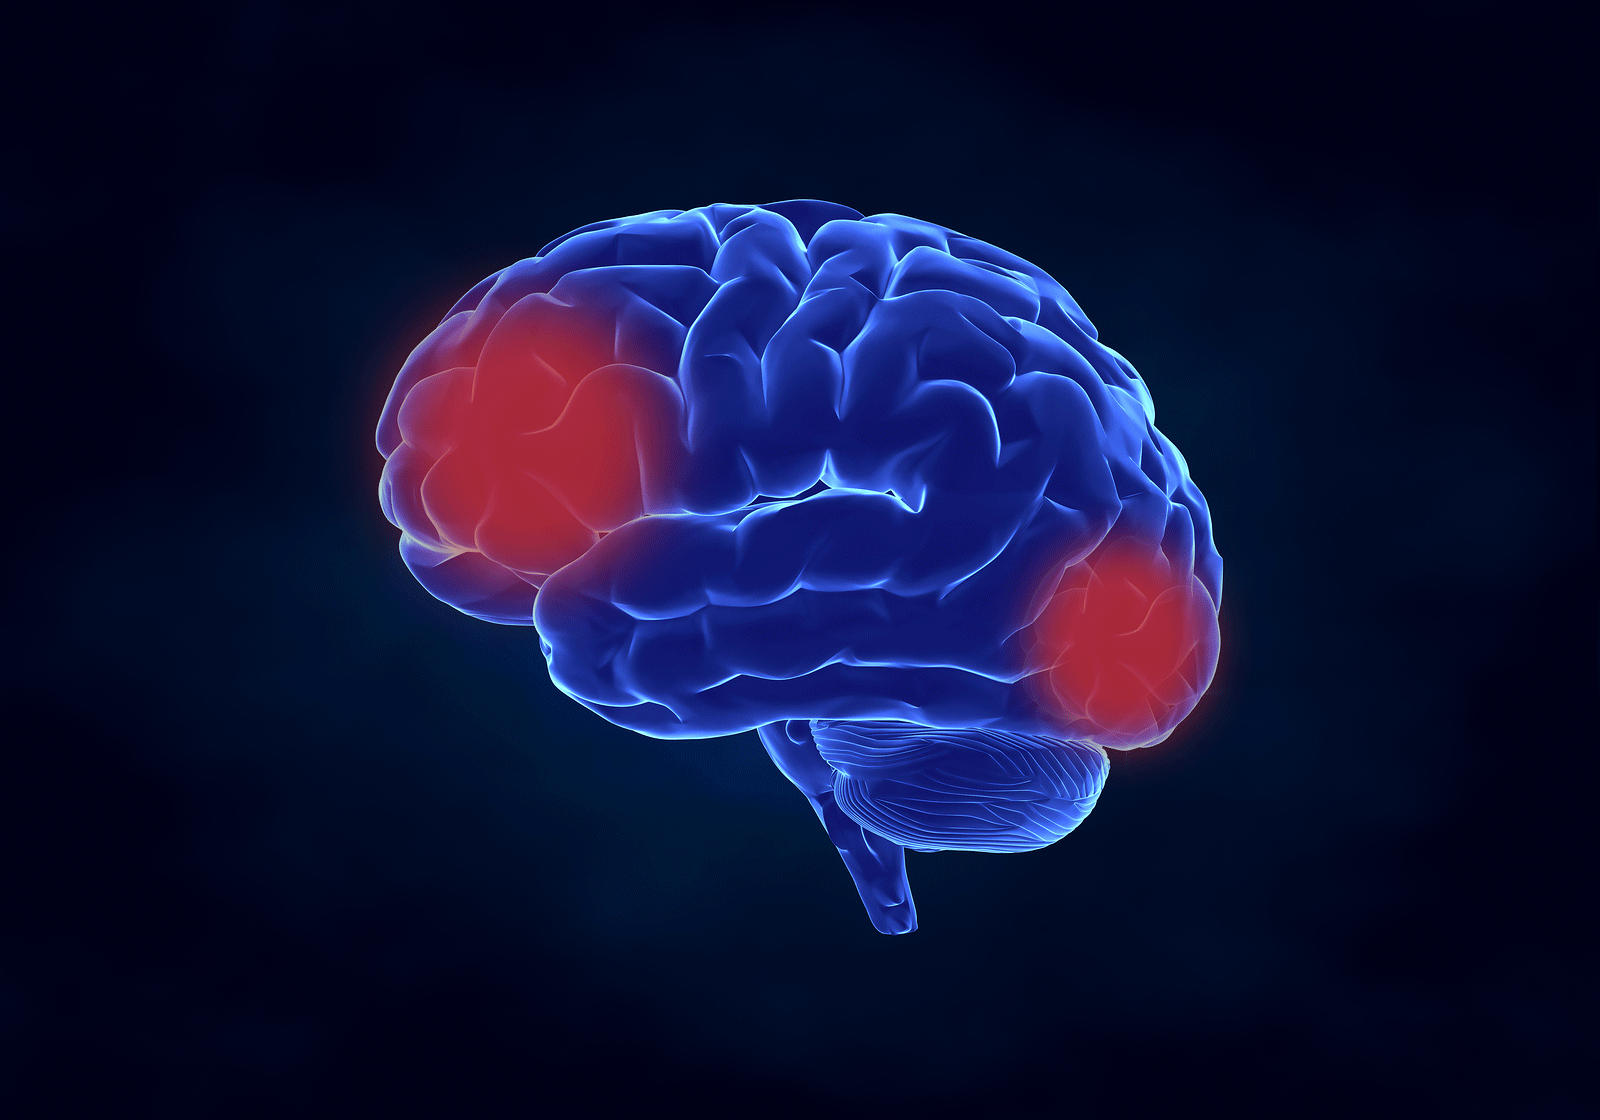
\includegraphics[scale=0.09]{coup-contrecoup.png}
	\caption{Coup/Contrecoup Impacts}
\end{figure}

One of the better known head mechanical processes up to this date was the coup/contrecoup system. This system describes the way in which the brain moves inside the skull during an impact. Referring to Figure 1, let us take an example in which a force is applied to the front of the head (forehead area). The force is directly applied to the front of the skull, which causes the skull to projectile backwards and impact with the front of the brain. This domino effect causes the brain to projectile backwards until the back of the brain impacts with the back of the skull. For a purely translational impacts, as Holbourn states, coup/contrecoup impacts are negligable. As the first publication attempting to mechanically analyze brain injuries, this assumption was a good starting place. However, this assumption is easily refutable when considering that the head rotates around a point located at its base (the neck area). Thus, even if the initial impact was purely translational, the rotation added to the system due to the head's point of rotation would create a shear-strain value that increases as continued rotational impacts occur with continued coup/contrecoup impacts. So, even though a rotational initial impact will create the most deformation within the brain, even a purely translational impact will create some deformation.

\subsection{Modelling the brain}

In 1954, Kornhauser modeled the brain as a second-order mass-spring system. He represented the brain as many components connected by springs. This can be portrayed using Figure 2, where you could assign individual masses in the spring system to different ``nodes" in the brain (sections of the brain). Let's say for this example that masses $m_1$ and $m_2$ are the left and right hemispheres of the brain, respectively. The relationships between different nodes within the brain are represented by sprints with corrresponding sprint constants $k_1$, $\kappa$, and $k_2$. The relationship between the skull and left hemisphere would thus be represented by the spring with spring constant $k_1$, and so on for the rest of the system. In Kornhauser's model, he considers movements of the brain in which the masses will not move due to either extremely low or high acceleration. In this case, the springs will be overloaded such that they will not have time to compress, thus will not cause any displacement to the nodes within the system.
% In 1954, Kornhauser modeled the brain as a second-order mass-spring system. He represented the brain as many components connected by springs, as shown in Figure 2. For example, the first mass, $m_1$, could be the left hemisphere of the brain and the second mass, $m_2$, the right hemisphere. On an impact to the left side of the head, the leftmost spring acts with spring constant $k_1$ into mass $m_1$, thus enacting the rest of the system (the middle spring, mass $m_2$, and the right spring). The masses act as ``nodes" that represent different parts of the brain, which can have completely different physical characteristics (density, bulk modulus, shear modulus, etc.); the springs act as the compressability between nodes (relatively low).

\begin{figure}
	\centering
	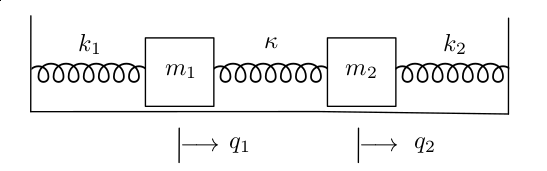
\includegraphics[scale=0.4]{coupledmasssystem.png}
	\caption{Coupled Mass System\cite{Schramm2018}}
\end{figure}

Kornhauser uses sensitivity curves shown in Figure 3 (velocity change vs. average acceleration) to allow for such low or high acceleration impacts to be considered within the system. Since head impacts are highly transient events, often occurring within 100 milliseconds, high accelerations are common and must be accounted for in any subsequent models. The fundamental part of the sensitivity curve is that there is a ``go" zone and a ``no go" zone; if the velocity change and average acceleration of a certain node in the brian are too low, then the node of the brain will not move. Likewise, if the velocity change is high and the average acceleration is low (or vice versa), the node will not move. If both components are high, there will be movement (or actuation) of the node.

\begin{figure}
	\centering
	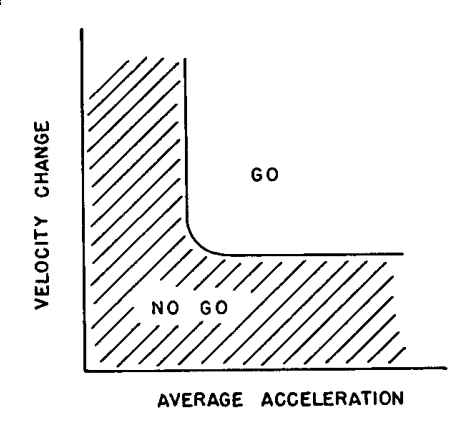
\includegraphics[scale=0.4]{sensitivitycurve.png}
	\caption{Sensitivity Curve\cite{Kornhauser1954}}
\end{figure}

\begin{equation}
	\frac{1}{2}G_0 = \frac{1}{2}\omega^2 (x_p + x_0)
\end{equation}

Equation 1 is the Kornhauser model; $G_0$ is the steady acceleration required to produce $x_0$, $\omega$ is the eigenfrequency that the system vibrates, $x_p$ is the preset deflection of mass (predisposed position), and $x_0$ is the specified travel of mass to actuate inertia mechanism (how far the mass travels from $x_p$).

\subsection{Recent Research}

In the past two decades, the best research done on head impacts and their influence on mTBI has been done by finding correlation between certian head impact characteristics and mTBI (concussion) status. Most of the research includes correlating the rotational acceleration of the head upon impact to the concussive status of the subject. This research is essentially an extension of the claims made by Holbourn in 1943; rotational components influence more damage to the brain than translational components. 

\begin{figure}
	\centering
	\begin{tikzpicture}
		\node [inner sep=0pt,above right]
       		{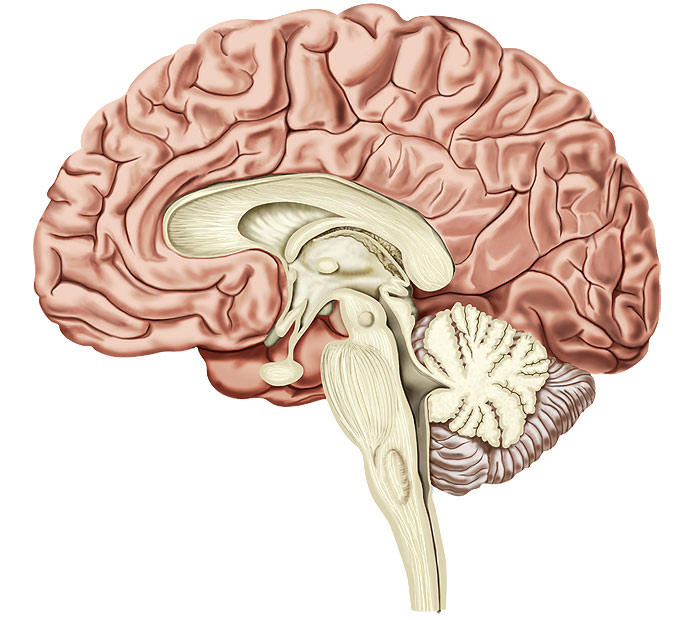
\includegraphics[scale=0.3]{brain.jpg}};
		\draw[->] (2,1.4) -- (3.5,4.5);
		\node (none) at (2,1.1) {Corpus Callosum};
		\node (none) at (2,0.8) {(Periventricular Region)};
	\end{tikzpicture}
	\caption{Location of Corpus Callosum within the Brain}
\end{figure}

Advances in imaging technology and technique, especially with the MRI, has led to the conclusion in other publishings that axonal injury is a good predictor for TBI and mTBI. Axonal injury is the damaging of axons within the brain, most commonly in the area called the corpus callosum (Figure 4). This landmark of the brain has the highest density of axons, so any axonal injury that occurs to this area will cause a greater influence to symptoms than axonal injury to another area of the brain. The corpus callosum sits within the white matter area of the brain known as the periventricular region (the region peripherally located from the ventricles). It offers protection for this ventricular region. The ventricles of the brain allow for the circulation of cerebrospinal fluid, so the region itself (without the fluid) is hollow. Moving radially outward from the white matter of the brain is the gray matter region, which is slightly more dense than the white matter region. When a shear wave travels through the brain, the wave will be most likely to cause shearing along the crossing from a low-density to high-density mass, or vice versa. This is what happens when travelling from low-density white matter to the high-density corpus callosum. Rotational acceleration components added to these shear waves further influence the action of shearing. Shearing is visualized in Holbourn's 1943 paper using the analogy of a deck of cards. If you have the deck with all cards stacked on one another with a circle drawn on the side of the cards (so that each card is marked on its side), shearing will deform the circle into an oval shape as the cards slide over one another.

\begin{figure}
	\centering
	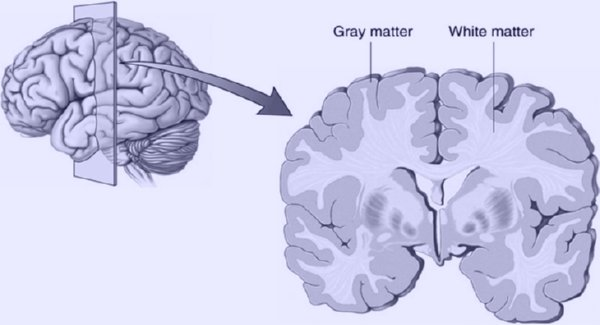
\includegraphics[scale=1.7]{brainmatter.jpg}
	\caption{Gray Matter and White Matter}
\end{figure}

\section{\label{sec:level3}Finite Element Model}

In 2014, a study was done using head impact data and a finite element model that inputs skull displacement data and outputs brain displacement data. The method in which the data was captured for this study allowed for six degrees of freedom (DOF) to be measured; the first study of its kind to measure a true six DOF (three translational and three rotational DOF). The regulatory safety standards for head injury have traditionally only used three DOF, translation-only kinematic criteria\cite{Hernandez2014}, even though the three DOF criterea has been proven to be a poor predictor of mTBI (as it does not capture the full picture of head injury).

\subsection{Methods}

The study began by outfitting football players with special mouthguards, shown in Figure 6. The mouthguard was given the capability of measuring a full six DOF by instrumenting it with a tri-axis accelerometer to measure translational acceleration (anterior to posterior, left to right, superior to inferior) as well as a tri-axis gyroscope to measure rotational acceleration (frontal, sagittal, and transverse planes). The accelerometer and gyroscope combination made this the first device to measure a true six DOF. All devices before that have offered six DOF have approximated the rotational components using the translational components, which does not present an accurate data set. The main assumption with the instrumented mouthguard in this study is that the skull is a perfectly rigid body, which does not bend or stretch from the jaw to the main skull area that houses the brain.

Time-stamped, high-definition video was taken at the athletic event so that the time captured from the mouthguard could be synced with the video. Head impacts were noted on the video, and the corresponding kinematic data from the mouthguards were taken.

\begin{figure}
	\centering
	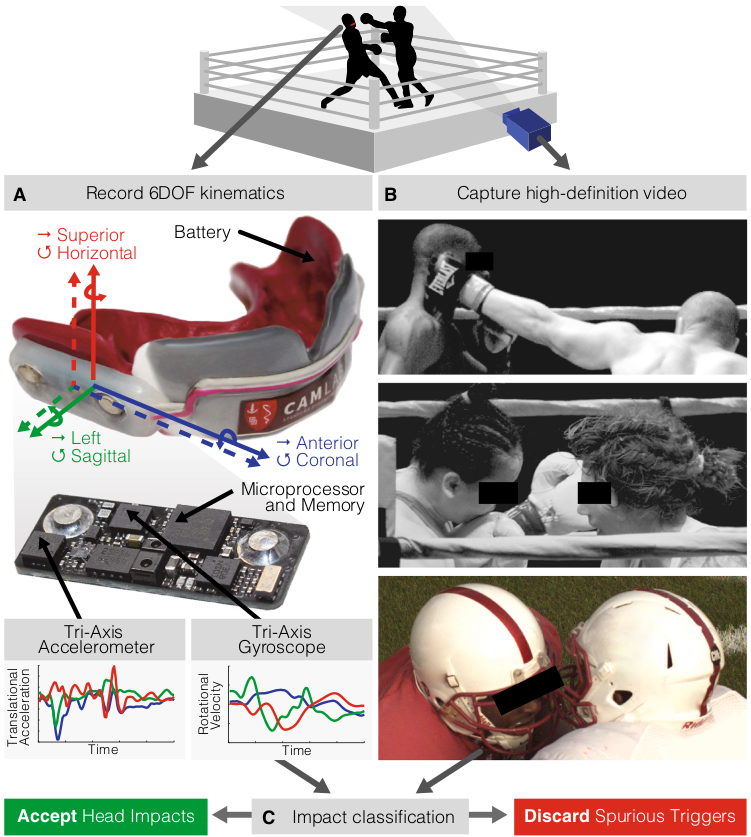
\includegraphics[scale=0.2]{mouthguard.png}
	\caption{True Six Degrees of Freedom Measuring Mouthguard}
\end{figure}

\subsection{Finite Element Model}

In order to obtain brain displacement data, a brain finite element developed at the KTH Royal Institute of Technology in Stockholm, Sweden\cite{Kleiven2005} was used. The model uses an average adult male human head model, developed in LS-DYNA in Livermore, CA. The adult head model incorporates the scalp, skull, brain (white matter, gray matter, and ventricles), meninges, cerebral spinal fluid, and veins. The brain-skull interface is modelled using tied-node contact, which restricts the node (brain) to moving with the master surface (skull). Therefore all initial skull actuations are equal to initial brain actuations. With the six DOF data from the instrumented mouthguards, the brain finite element model was put into use to obtain brain displacement data. The shear-strain was calculated from this data using the basic strain equation $\epsilon = \frac{\Delta l}{l}$, where $\epsilon$ is the strain, $\Delta l$ is the displacement, and $l$ is the original position. The strain is calculated for each chosen node in the brain and shown in Figure 7.

\begin{figure}
	\centering
	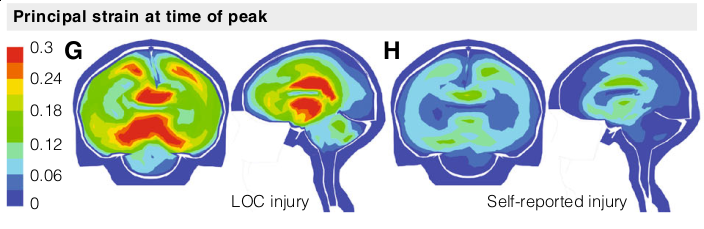
\includegraphics[scale=0.325]{axonalstrain.png}
	\caption{Peak Axonal Strain in the Brain}
\end{figure}

The data points were separated based on the individual receiving the impact. There were 100 total impacts randomly chosen from the entire data set, 2 of which an injury (TBI or mTBI) occurred. In Figure 8, the peak strain for each individual head impact is shown. For both cases that resulted in injury, the peak strain occurred in the corpus callosum. This is consistent with the previously published information declaring that strain in the corpus callosum causing axonal damage was the best predictor of TBI and mTBI.

\begin{figure}
	\centering
	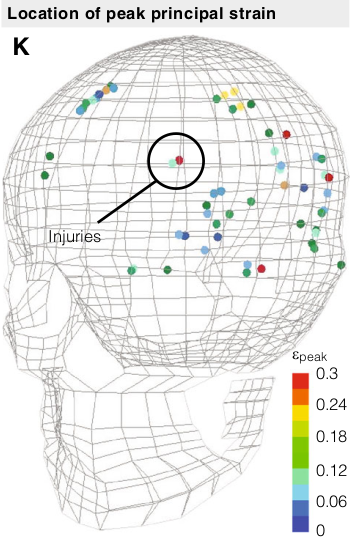
\includegraphics[scale=0.4]{peakstrain.png}
	\caption{Peak Strain Localized for Each Head Impact}
\end{figure}

\section{\label{sec:level4}Dynamic Mode Decomposition}

Studies done on the mechanics of head impacts and their ability to predict TBI have, for the most part, used relatively deterministic methods. That is, the methods used in these studies have attempted to show something that is already assumed to be true. None of the studies give any underlying characteristics that can be used to define the system as a whole. Dynamic mode decomposition (DMD) is a method often used in fluid mechanics to analyze the dominant characteristics of fluid systems to understand the underlying physics of the system.

\subsection{Introduction}

DMD was first introduced in 2010 by Peter Schmid as a method of extracting ``coherent features" that are ``essential to our understanding of fluid-dynamical and transport processes."\cite{Schmid2010} The data used for the DMD process can be either experimentally (physically measured) or numerically (from a model) obtained. The DMD analysis acts as a global stability analysis, which gives the global characteristics of the system. From this global stability analysis, a numerical analysis is used to extract the dominant, dynamical features of the system (further decomposition). In Figure 9, a common fluids mechanics example is shown. The dominant characteristics of this dynamic system are already visible. DMD will further decompose this system so that the extra noise in the system is removed. In Figure 10, the DMD analysis of this example is shown. The dominant features of the system are easily seen in the figure; the first picture being the first mode, the second picture of the second mode, and the third picture of the third mode. The first mode of this decomposition, like the first mode of any dynamical system, is the simplest form. 

\begin{figure}
	\centering
	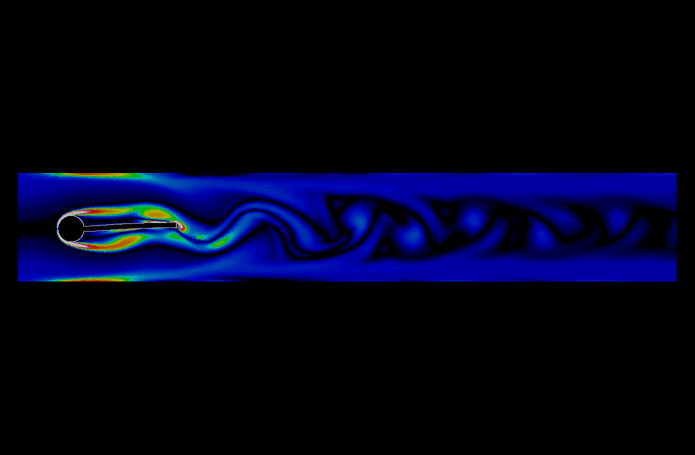
\includegraphics[scale=0.3]{flow-37.png}
	\caption{Vortex Shedding (Fluid Mechanics Example)}
\end{figure}

\begin{figure}
	\centering
	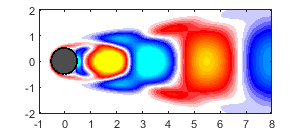
\includegraphics[scale=1]{examplemodes1.png}
	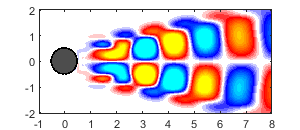
\includegraphics[scale=1]{examplemodes2.png}
	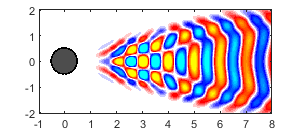
\includegraphics[scale=1]{examplemodes3.png}
	\caption{Output of DMD}
\end{figure}

\subsection{Method of DMD}

The method of DMD begins with expressing the flow field as a large matrix $X_1^N$ of size $m \times n$, given in Equation 2. For the a fluids example, the flow field is constructed by taking a snapshot of the fluid at small time steps $\Delta t$. In the matrix $X_1^N$, $x_1$ is the fluid at time $t_1$, $x_2$ is the fluid at time $t_2$, and so on. So each column of our flow field matrix is an individual snapshot of a fully developed flow field after a certain total time $t$. For highly transient events, such as a head impact, the time $t$ over which the flow field becomes fully developed is small, so the time between snapshots $\Delta t$ will be small. There will also be fewer snapshots, reducing the width of the matrix $X_1^N$.

\begin{equation}
	X_1^N = \{ x_1, x_2, x_3, ..., x_N \}
\end{equation}

Each column of $X_1^N$ is constructed using the spacial characteristics of the fluid field. For example, in the matrix below, $x_{1a_x}$ is the position of a certain node $a$ measured in the $x$ direction. The next matrix component in that $x_1$ column, $x_{1a_y}$, is the position of the same node in the $y$ direction, and so on for all nodes in the fluid of interest. The fluid field matrix can be constructed using two types of data, analytical or experimental. Analytical data is obtained by using a mathematical model in which nodes are predefined. Experimental data is obtained through the physical measurement of node position in a fluid. For example, experimental data could be taken from Figure 9 by fixing your focus on a point in the fluid at time $t=0$, then measuring the spatial position as it changes with changing time $t$. With this experimental form of data, the number of nodes defined could be infinite. The matrix $X_1^N$ that is thus formed from all snapshots $n$ and nodes $m$ is a tall, skinny matrix with $m > n$.

% For experimentally obtained data, there could be an infinite number of nodes, depending on how many nodes have been defined by the observer doing measurements. In order to best describe the flow field, a greater number of nodes within the fluid of interest will be defined. For the human brain, the minimum nodes that could be defined would be all of the major landmarks within the brain, such as the white matter, gray matter, corpus callosum, ventricle area, etc. The matrix $X_1^N$ that is thus formed from all snapshots $n$ and nodes $m$ is a tall, skinny matrix with $m > n$.

$$
\begin{bmatrix}
    			x_{1a_x}       & x_{2a_x} & x_{3a_x} & \dots & x_{na_x} \\
    			x_{1a_y}       & x_{2a_y} & x_{3a_y} & \dots & x_{na_y} \\
    			x_{1a_z}       & x_{2a_z} & x_{3a_z} & \dots & x_{na_z} \\
    			x_{1b_x}       & x_{2b_x} & x_{3b_x} & \dots & x_{nb_x} \\
    			\vdots & \vdots & \vdots & \ddots & \vdots \\
    			x_{1z_z}       & x_{2z_z} & x_{3z_z} & \dots & x_{nz_z}
\end{bmatrix}
$$

The next step of DMD is finding a linear mapping $A$ that takes the first snapshot $x_1$ and projects it into the second snapshot $x_2$. This linear mapping also takes the second snapshot into the third snapshot, and so on until it takes $x_{n-1}$ into $x_n$. The mapping $A$ is a linear best fit that is applied to the entire flow field $X_1^N$. For a linear system, the matrix $A$ is a linear best fit; for nonlinear systems, the matrix $A$ is linear tangent approximation of the system. A perfectly linear system will allow for a constant mapping of $A$ across all snapshots in the flow field. For all other systems, the matrix $A$ is assumed to be a constant mapping. In our case, the brain is a nonlinear system since the material (as a whole) is nonhomogeneous.

\begin{equation}
	x_{i+1} = A x_i
\end{equation}

This constant mapping assumption allows for the snapshots to be written as a linear combination of $A$, in the form of a Krylov sequence, given in Equation 4. A Krylov subspace generated by matrix A and vector x of dimension N is the linear subspace spanned by the images of x under the first K powers of A. This Krylov sequence is written in the form that writes each snapshot with respect to $x_1$, the first snapshot in the sequence.

\begin{equation}
	X_1^{N} = \{ x_1, Ax_1, A^{2}x_1 ...,A^{N-1}x_1 \}
\end{equation}

The goal at this point is to find the dominant characteristics of matrix $A$, such as the eigenvalues and eigenvectors, that will allow for the formulation of a decomposed flow field. 

\subsection{Extraction Techniques}

The extraction of dominant characteristics of $A$ is almost always necessary because there is often not enough computational resources to capture such characteristics of a matrix of size $m \times n$, where $m$ is very large. Extraction techniques such as the  proper orthogonal decomposition and singular value decomposition are used to decompose the $A$ matrix further so that the dominant characteristics can be found of a decomposed matrix $S$ and used to approximate the characteristics of $A$.

Proper orthogonal decomposition extracts the dominant characteristics of $A$ based on the system's steady-state response (when the system has reached equilibrium). Since POD uses an energy-ranking system to find the steady-state response, it disregards many spacial characteristics (like phase information) that disables this method from finding spatial and temporal displacements for the system. For this reason, the POD method was not used in the DMD analysis.

Singular value decomposition is a method that produces a companion matrix that has the exactly the same dominant characteristics as matrix $A$. It uses a ranking system to find the dominant components of the flow field matrix in order to orthogonalize the companion matrix $S$ to find a simplified matrix $\tilde S$ that has the same characteristics of $A$. This is the preferred method for DMD since the orthogonalizing process neutralizes the high-ordered Krylov sequence.

\subsection{Method of SVD}

The method of SVD first involves writing the flow field column at some time $t$ in terms of the snapshot directly before it, at time $t - \Delta t$ using the companion matrix S (Equation 5).

\begin{equation}
	X' = SX
\end{equation}

\begin{equation}
	X = U \Sigma V^*
\end{equation}

Equation 6 represents the ranking system that is the main part of SVD. In this equation, the matrix $U$ is the ranked vector columns of our flow field $X$. This matrix is used to narrow down our flow field into its simplest components; if we can represent our flow field with the first 5 or 10 vector columns of $X$ instead of hundreds of vector columns at all possible snapshots, this matrix will represent those 5 or 10 pieces. The $U$ matrix is often called the left singular vectors of $X$. 

The matrix $V^*$, often called the right singular vectors of $X$, is a complement to the matrix $U$. $V^*$ ranks the most important components of each vector column of $X$ as a way to narrow down on nodes within our system that either do not change or don't contribute significantly to the flow field. This matrix $V^*$ aids in reducing the height of the matrix $X$. For our brain system, this process of reducing the number of nodes will likely take out areas of the brain that do not displace during a head impact. This will include mostly areas of gray matter that, according to our finite element model, are defined by tied-node contact, and thus move exactly with the skull.

The matrix $\Sigma$ gives the strength ranking of each vector column in $X$ in an orthogonalized form (the dominant vectors that contribute to the system the most and all non-zero components of matrix are along the diagonal). For example, the first component ($1 \times 1$) will be the ranking ``score" of the first vector column of $X$. If the second vector column of $X$ is more significant than the first, the $2 \times 2$ component of $\Sigma$ will be greater than the $1 \times 1$ component. This continues for all vector columns defined in $U$.

The matrix below gives the general shape of the $U$, $\Sigma$, and $V^*$ matrices, respectively. As mentioned above, the $U$ matrix takes $X$ and reduces the number of snapshots included, thus creating a tall and skinny matrix of size $m \times r$. The matrix $\Sigma$ is an orthogonalized matrix with rankings for each significant vector column in $U$, so the matrix is of size $r \times r$. The matrix $V^*$ is in the transpose form, so it is long and short in size ($r \times n$). The resulting size of $U \Sigma V^*$ is $(m \times r)(r \times r)(r \times n) = (m \times n)$.

$$
\begin{bmatrix}
	\vdots & \vdots & \vdots  \\
	\vdots & \vdots & \vdots  \\
	\vdots & \vdots & \vdots  \\
\end{bmatrix}
\begin{bmatrix}
	\vdots & \vdots & \vdots  \\
\end{bmatrix}
\begin{bmatrix}
	\hdots & \hdots & \hdots  \\
\end{bmatrix}
$$

Next, we use Equation 5 to rewrite $X'$ in terms of $X$ given in Equation 6. Since the goal of this SVD approach is to solve for the dominant characteristics in our companion matrix $S$, we want to isolate this matrix.

\begin{equation}
	X' = S U \Sigma V^*
\end{equation}

The companion matrix $S$ is isolated by using the properties of the SVD matrices. $U$ and $V^*$ are unitary matrices, that is $U^*U=I$ and $V^*V=I$, where $I$ is the identity matrix. With this in mind, $S$ can be isolated by mutliplying each side by $U^*$ and $V$. Since $\Sigma$ is an orthogonalized matrix, $S$ can be isolated by multiplying each side by the inverse $\Sigma^{-1}$. The end result is an isolated companion matrix $S$ of size $m \times n$. This is still a relatively large matrix, however, and can be reduced further into $\tilde S$ by projecting $U$ onto $S$. This process orthogonalizes the matrix $S$, reduces its size, as well as fixes the problem of linear dependence due to the high power iterations of the Krylov sequence.

\begin{equation}
	U^* X' V \Sigma^{-1} = U^* S U = \tilde S
\end{equation}
		
Now that we have our reduced companion matrix $\tilde S$, we can extract our dynamic characteristics. The eigenvalues and eigenvectors are derived from the eigenvalue equation, given in Equation 9, where $\lambda$ is the eigenvalues and $W$ is the eigenvectors of $\tilde S$.

\begin{equation}
	\tilde S W = W \lambda
\end{equation}

The spatial displacements of nodes within our system, which use our eigenvectors $W$ is given by Equation 10, which is derived in Schmid's 2010 paper.

\begin{equation}
	\phi = X' V \Sigma^{-1} W
\end{equation}

Putting it all together, our decomposed flow field is represented by Equation 11. Our spatial displacements are described by $\phi_n$, our temporal modes are described by $e^{\lambda_n t}$, and our amplitude of flow is represented by $a_n$, which is solved for using initial conditions at time $t=0$.

Looking back to Figure 10, these flow fields represent our $U(x,y,z,t)$ from Equation 11. A simplified flow field with less noise that only includes the significant, dynamic structures of our system of interest. 

\begin{equation}
	U(x,y,z,t) = a_n e^{\lambda_n t} \phi_n(x,y,z)
\end{equation}

\section{\label{sec:level5}Implications}

Figure 11 shows the flow field of our brain system after the DMD and SVD process. The snapshots given are of time $t$ from 25ms to 65ms with a time step $\Delta t$ of 10ms. We can see from comparing the first mode with the third mode that the displacements are greater for the first mode. This pattern continues for higher modes. This means that our system is dominated by low frequencies. Figure 12b shows that about 75\% of the total brain displacement energy can be represented by all frequencies up to and slightly past the first mode at 33Hz. 

\begin{figure}
	\centering
	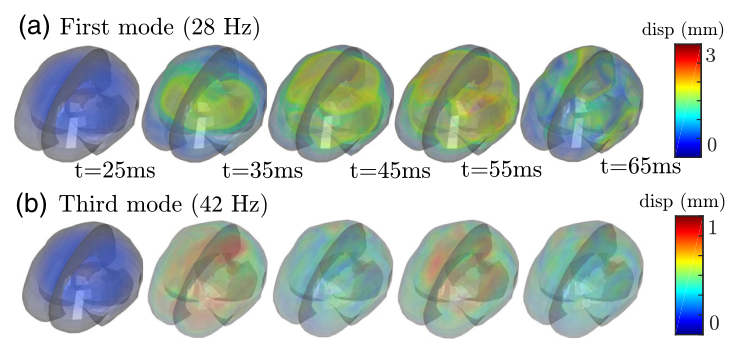
\includegraphics[scale=0.3]{modes.png}
	\caption{Dynamic Modes within the Brain}
\end{figure}

In Figure 12a and 12c, the frequency of the system is plotted against modal amplitudes and peak principal strains, respectively. The modal amplitudes are given from Equation 11 and the peak principal strains are calculated using the strain equation from the displacement data. These two sets of data (modal amplitude and peak principal strain) were normalized with one another by dividing each one by the average rotational acceleration for each head impact in the group. The normalization process allows for the modal amplitudes to be directly compared to the peak principal strain. The form that these two graphs take is very similar, with the modal amplitudes fitting consistently within the error of the peak principal strain (gray area on Figure 12c). With these two normalized values being consistent with one another, the DMD analysis shows that there are well defined modes that, at low frequencies, influence the strain inflicted on the brain. 

\begin{figure}
	\centering
	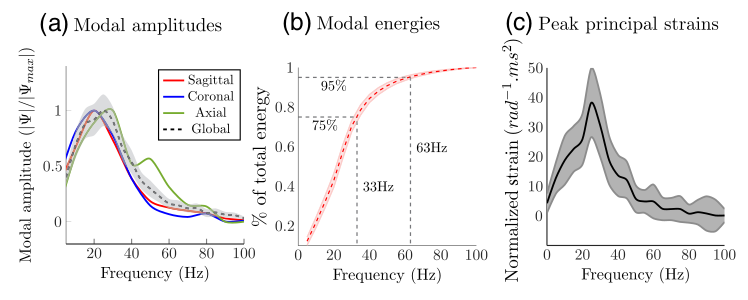
\includegraphics[scale=0.3]{strainnormalization.png}
	\caption{(a) Modal amplitudes of the system given by Equation 11. (b) Modal energy, 75\% of which can be represented by frequencies under 33 Hz. (c) Peak principal strain across the brain, amplified around 28 Hz.}
\end{figure}

Going further, a local analysis was done looking at the peak principal strain at individual parts of the brain, shown in Figure 13. The individual resonant frequency for different parts of the brain is shown on the same peak principal strain graph from Figure 12c. Not surprisingly, the corpus callosum (labeled ``CC" in Figure 13) had the highest strain value out of any other node within the brain. The white matter area (labeled ``WM") was a close second, which makes sense since this area is radially adjacent to the corpus callosum. This data is a confirmation that DMD modes contribute significantly to the peak strain that occurs in the brain, which occurs the most in the corpus callosum. This is also further evidence for the corpus callosum being an area of interest for predicting mTBI, confirming Hernandez's 2014 study. 

\begin{figure}
	\centering
	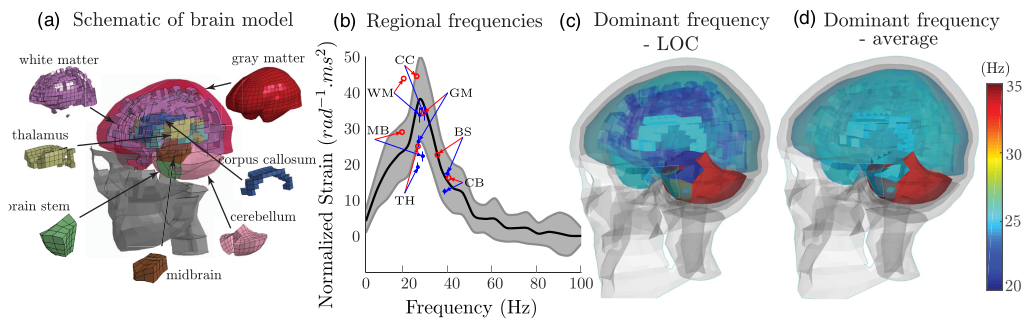
\includegraphics[scale=0.23]{localization.png}
	\caption{Strain Localization}
\end{figure}

\section{\label{sec:level6}Conclusion}

% introduction
% previous insights
% finite element model
% dmd
% implications

Traumatic brain injury and concussions pose a risk with steep consequences. The ability to predict a concussion before symptoms show would be an important tool to have in reducing recovery times and preventing further injury. This process all starts with the brain finite element model developed by the Swedish team at KTH Royal Institute. With the brain finite element model, we are able to use skull displacement data to accurately predict how different nodes within the brain will move upon impact. Using this brain displacement information, a flow field matrix can be developed, showing the position of each node in the brain throughout the duration of the impact. With the help of DMD and SVD, patterns within the brain system are found during a head impact that can be used to aid in predicting concussions. The DMD process finds a linear mapping matrix $A$ that maps each snapshot in the flow field matrix to one another. The SVD process finds the companion matrix $\tilde S$ that has the same eigen-characteristics as $A$ with a significantly reduced-dimensionality. 

The results of DMD analysis on head impact data has proven the existance of dominant modes in the brain. This low-frequency dominated system is most prone to shearing in the corpus callosum region, the area with the highest density of axons in the brain. The dominant frequency of the system (~30 Hz) was shown to have correlation with the modal amplitude (Equation 11) and the peak strain on the system (Figure 12). Looking to the future development of this research, reduced-order models can be created that mimick low-frequency dynamics. That way, a numerical approach to calculating brain displacements will be available instead of the experimental finite element model. This would allow for technology to be created that could calculate in real time the strain put on the brain based on skull displacement data (all using a reduced-order model and DMD analysis). This could be in the form of an advanced mouthguard like the one used in Hernandez's 2014 study, where the mouthguard measures the skull displacements and then the data is immediately used to calculate strain in the case of an injury to an athlete.

There are a few limitations to this research. First, the brain finite element model has not been validated for in vivo brains, only for cadavers. This is due to the fact that no living human would be willing to offer their brain to sustain numerous impacts just for validation of this finite element model. It is unclear if an in vivo brain will produce different results from a cadaver brain. The obvious limitation to this idea is that it would only apply to athletes or professions that might wear mouthguards on a regular basis. Second, the DMD process produces a linear tangent {\it approximation} since the brain is a nonlinear, nonhomogenous system; this limits the accuracy of the results. Third, the head impact data used was obtained only from impacts sustained by football players in a practice setting. This could limit the variability of the type of impact sustained. This is, however, a great starting point for this research since concussions in football are so common. Also, the head mechanics for other impacts will follow relatively similar mechanics with varying initial points of impact.

% \nocite{*} % includes all citations in .bib file
\bibliography{main.bib}% Produces the bibliography via BibTeX.

\end{document}
%
% ****** End of file aipsamp.tex ******
